\subsection{Hustota hladin $f$-rozměrného oscilátoru}
	\begin{enumerate}
	\item
		Spočítejte hustotu hladin $\rho_{0}(E)$ izotropního $f$-rozměrného harmonického oscilátoru.

	\item
		Částice se pohybuje v potenciálu podle obrázku: jedná se o dvě $f$-rozměrné izotropní kvadratické jámy, jejichž minima se nacházejí na souřadnicích
		\begin{equation*}
			\vector{M}_{1}=(\vector{q}=\vector{0},E=\vector{0})\,,\qquad \vector{M}_{2}=(\vector{q}=\vector{q}^{(0)},E=E^{(0)})\,,\qquad E^{(0)}>0\,.
		\end{equation*}
		Určete hustotu hladin $\rho(E)$ v intervalu energií $E\in(0;E^{(1)})$, přičemž předpokládejte, že $E^{(1)}>E^{(0)}$ a že obě jámy jsou pod energií $E^{(1)}$ oddělené.
		
	\item
		Funkce $\rho(E)$ bude neanalytická v bodě $E^{(0)}$. 
		Určete, v kolikáté její derivaci se poprvé neanalytičnost projeví jako nespojitost.
		
	\end{enumerate}
	
	\begin{figure}[!htbp]
		\begin{center}
			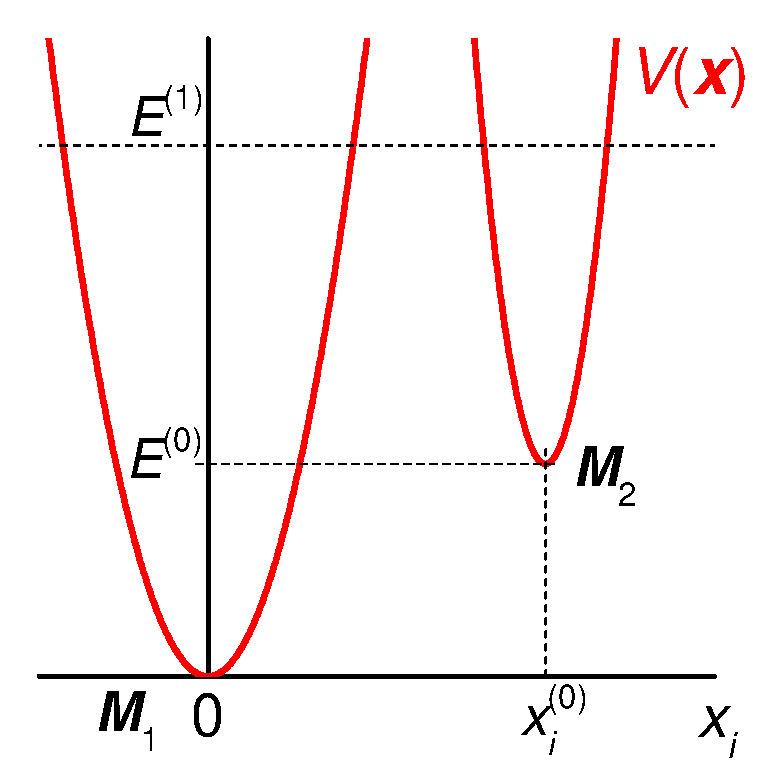
\epsfig{file=dwdensity.eps,width=0.5\linewidth}
			\caption{
				Dvoujámový potenciál: řez podél jedné ze souřadných os $q_{i}$, $i\in\left\{1,2,\dotsc,f\right\}$.
			}
		\end{center}
	\end{figure}
